\documentclass{standalone}

\usepackage{tikz}
\usepackage{standalone}
\usetikzlibrary{calc}

\begin{document}

    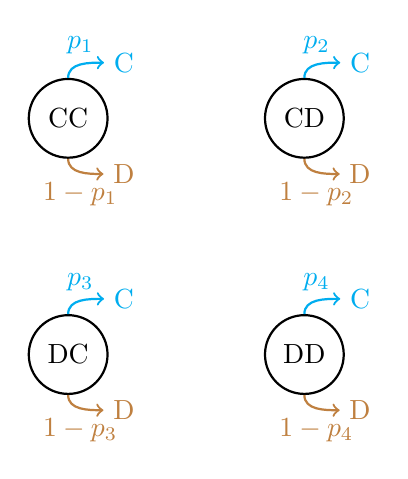
\begin{tikzpicture}

    \tikzstyle{state}=[minimum width=1cm, font=\boldmath];
    

	\node[circle, draw, thick] (0) at (0, 0) [state] {CC};
	\node[circle, draw, thick] (1) at (3, 0) [state] {CD};
	\node[circle, draw, thick] (2) at (0, -3) [state] {DC};
	\node[circle, draw, thick] (3) at (3, -3) [state] {DD};

	\node[above right of=0] (p1) {\textcolor{cyan}C};
	\node[below right of=0] (minus_p1) {\textcolor{brown}D};

	\node[above right of=1] (p2) {\textcolor{cyan}C};
	\node[below right of=1] (minus_p2) {\textcolor{brown}D};

	\node[above right of=2] (p3) {\textcolor{cyan}C};
	\node[below right of=2] (minus_p3) {\textcolor{brown}D};

	\node[above right of=3] (p4) {\textcolor{cyan}C};
	\node[below right of=3] (minus_p4) {\textcolor{brown}D};

	\draw (0) edge[cyan, out=90, in=180, ->, thick] node [above] {$p_1$} (p1);
	\draw (0) edge[brown, out=-90, in=180, ->, thick] node [below] {$1-p_1$} (minus_p1);

	\draw (1) edge[cyan, out=90, in=180, ->, thick] node [above] {$p_2$} (p2);
	\draw (1) edge[brown, out=-90, in=180, ->, thick] node [below] {$1-p_2$} (minus_p2);

	\draw (2) edge[cyan, out=90, in=180, ->, thick] node [above] {$p_3$} (p3);
	\draw (2) edge[brown, out=-90, in=180, ->, thick] node [below] {$1-p_3$} (minus_p3);

	\draw (3) edge[cyan, out=90, in=180, ->, thick] node [above] {$p_4$} (p4);
	\draw (3) edge[brown, out=-90, in=180, ->, thick] node [below] {$1-p_4$} (minus_p4);





    \end{tikzpicture}

\end{document}